\documentclass[12pt]{article}
\usepackage{mathtools}
\usepackage[utf8]{inputenc}
\usepackage[spanish,mexico]{babel}
\usepackage{graphicx}
%\graphicspath{ {\Users\Jose\Desktop\COMPUTACIONAL} }
\DeclareGraphicsExtensions{.png}
\title{Péndulo simple}
\author{Jose Pablo Salazar Velazquez}
\date{}
\usepackage{graphicx}
\begin{document}
\maketitle
   Describir el movimiento de un péndulo, mediante ecuaciones matemáticas, suele ser algo complicado. Se pueden hacer suposiciones que simplifican el análisis del problema. Para el caso del péndulo simple, permiten resolver analitacamente las ecuaciones de movimiento, para oscilaciones con un angulo incial pequeño.
    
    \section{Péndulo simple}
Al hablar de un "péndulo simple", simplemente nos referimos al análisis de un "pendulo real" en un sistema aislado, haciendo las siguiente suposiciones:
          \begin{itemize}
         \item La barra, cable, o hilo, del cual se sostiene la plomada, no tiene masa.
         \item La plomada, es una masa puntual.
         \item El movimiento, ocurre solamente en 2 dimensiones.
         \item El movimiento, no pierde energia debilo a la fricción o resistencia al aire.
         \item El campo gravitacional, es uniforme.
         \item El soporte, no se mueve.
       \end{itemize}
 La ecuación diferencial, que describe el movimiento del pendulo, es
 \begin{equation}
 \frac{d^2\theta}{dt^2} + \frac{g}{l}\sin\theta = 0
 \end{equation}
 

 Donde g es la aceleracion de la gravedad, l es la longitud del pendulo, y $\theta$ es el desplazamiento angular.
 Resolviendo para angulos pequeños, el periodo nos quedada:
 \begin{equation}
T \approx 2\pi \sqrt[]{\frac{l}{g}}
\end{equation}
\section{Codigo}
Este fue el código que se utilizó para resolver la practica:
\begin{verbatim}
import numpy as np
from scipy.integrate import quad
import matplotlib.pyplot as plt

#Constantes

g=9.81 
l= 3  
n= 1000
e=0.001 
T0 =np.linspace(e, (np.pi)-e, n)

#Integrales
I = [0 for i in range(n)]
E = [0 for i in range(n)]
T = [0 for i in range(n)]
To = 2.0 * np.pi*np.sqrt(l/g)

#Integrando
inte = lambda x, c : 1.0 /(np.sqrt(np.cos(x)-np.cos(c)))

for i in range(n):
    
    T1 = T0[i]
    I[i] , E [i] = quad(inte, 0, T1, args=(T1))
    T[i] = 4*np.sqrt(l/(2*g)) * I[i]
       
R=T/To

Tg= (T0*180.0)/np.pi 

#Graph
plt.plot(Tg, R, "go")
plt.grid()
plt.title("Error ")
plt.xlabel("Angulo")
plt.ylabel("Razon entre periodos")
plt.axis([0,180,1,5])
plt.show()
\end{verbatim}
Los resultados, que arrojo el programa, para n=100,500, y 1000, fueron los siguientes: \\
\subsection{n=100}
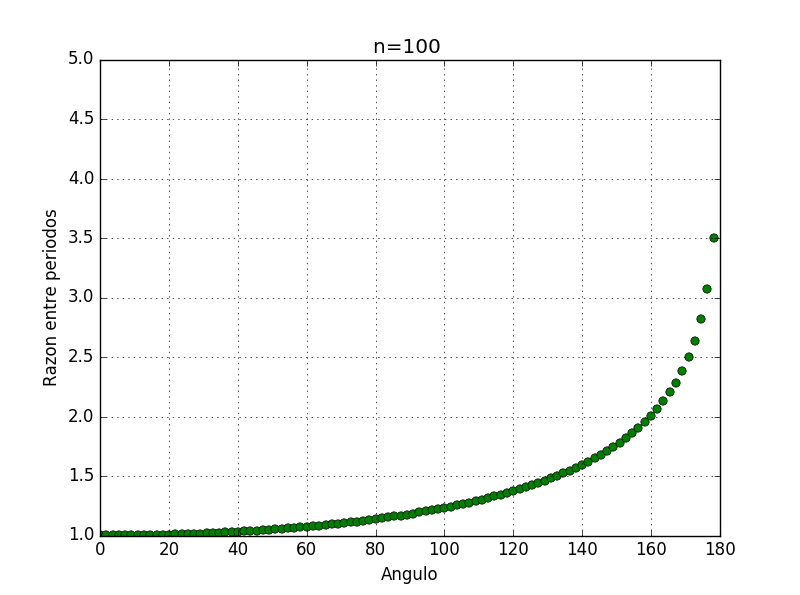
\includegraphics[width=9cm]{figure_1}
\\
\subsection{n=500}
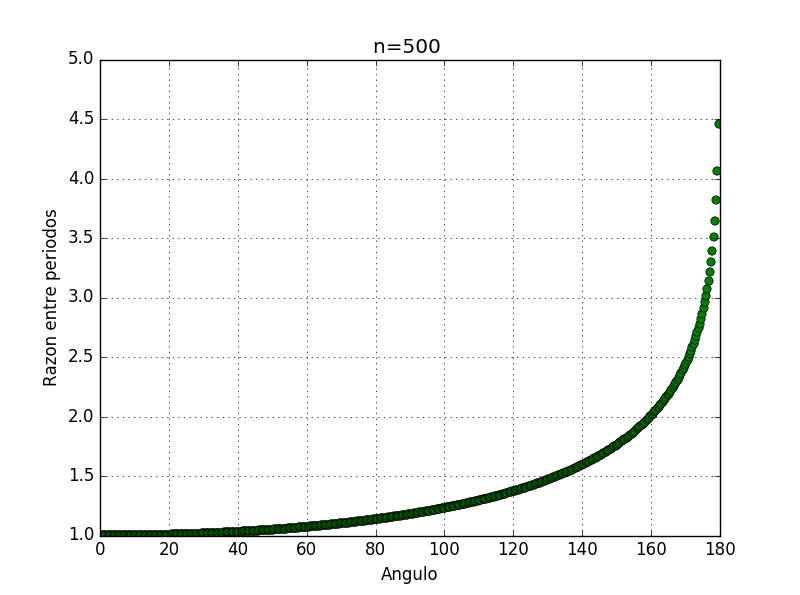
\includegraphics[width=9cm]{figure_2}
\\
\subsection{n=1000}
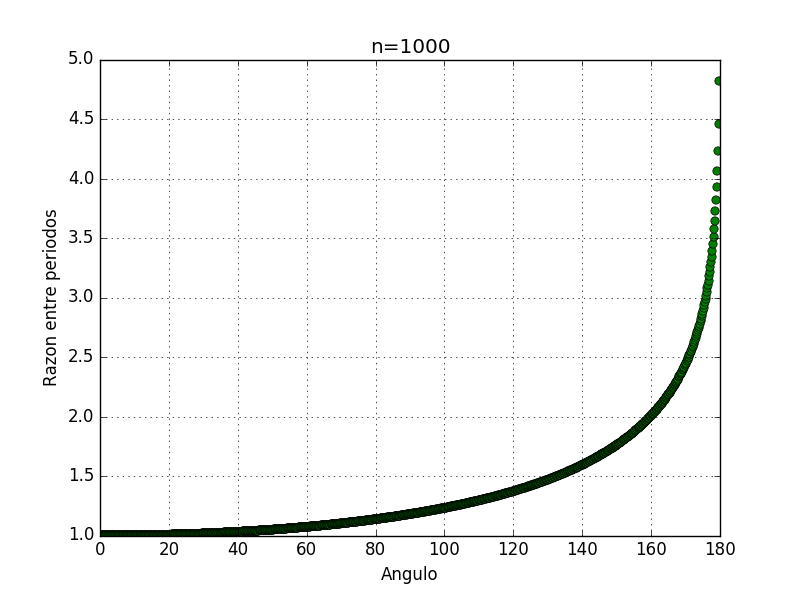
\includegraphics[width=9cm]{figure_3}
\\
\section{Referencias}
$ https://en.wikipedia.org/wiki/Pendulum_mathematics 
$\end{document}